\documentclass[a4paper,11pt]{article}
\usepackage[latin1]{inputenc}
\usepackage[T1]{fontenc}
\usepackage{bbm}
\usepackage{amsmath}
\usepackage{indentfirst}
\usepackage{fullpage}
\usepackage{url}
\usepackage{graphicx}
\usepackage[center,footnotesize]{caption}
\usepackage[section]{placeins}
\usepackage{subfig}
\title{Series 5}
\date{October 18, 2011}
\author{Genomics and bioinformatics - Week 5}
\begin{document}
\maketitle

%-----------------------------------------------------------------------------%
\section{Markow model}
Lorem ipsum.

%-----------------------------------------------------------------------------%
\section{Reading frame}
In this exercise you are given a nucleotide sequence which contains a coding region somewhere. You have to deduce what is the reading frame of this coding region.

The general procedure to find the right frame for reading a nucleotide sequence is to convert the nucleotide sequence into the corresponding possible amnio acid sequences and see which one makes the most sense. As you know, the base pairs are read three by three and translated into amino acids. One can hence read a sequence in three different ways: A, B and C.

\begin{figure}[h!]
	\centering
	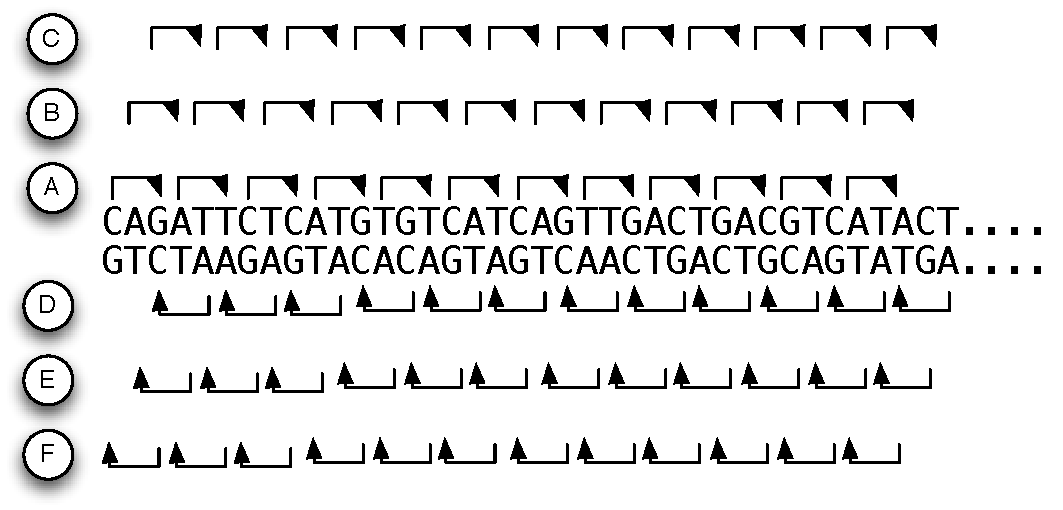
\includegraphics[width=0.7\textwidth]{reading_frame.pdf}
	\caption{Three possible reading frames.}
	\label{fig:gene_distribution_rib}
\end{figure}

So, to convert a base pair sequence (e.g. \texttt{CAGATTCTC}...) to a amino acid sequence (e.g. \texttt{GWLPHLQRI}...) you cut the base pair sequence in pieces of 3 nucleotides (e.g. \texttt{"CAG", "ATT",...}), and use a conversion table that links any possible 3mer to one of the 21 amnio acids. For instance, \texttt{CAG} codes for glutamine.

\subsection{All 3mers}
To build the conversion table that links 3mers to amino acids. We first need to build an exhaustive list of 3mers. Write the code that takes as input the list of the four base pairs and generates as output all the possible permutations of size three.
	
The output should start like this and have 64 elements:
	
\begin{verbatim}
    bases = ["t", "c", "a", "g"]
	codons = ['ttt', 'ttc', 'tta', 'ttg', 'tct', 'tcc', 'tca', 'tcg', 'tat', ...
\end{verbatim}

\subsection{3mer to amino acid}
We can now build a dictionary that links every 3mer to an amino acid. If you built the list correctly in the previous step, the corresponding amino acids are the following.

\begin{verbatim}
aminos = "FFLLSSSSYY**CC*WLLLLPPPPHHQQRRRRIIIMTTTTNNKKSSRRVVVVAAAADDEEGGGG"
codon_to_amino = {'aaa': 'K', 'aac': 'N', 'aag': 'K', 'aat': 'N', 'aca': 'T', ...
\end{verbatim}

\subsection{Sequence to protein}
You can now write the function that takes a nucleotide sequence as entry and outputs a protein sequence.

\begin{quote}
\begin{verbatim}
	def seq_to_prot(seq): ...........
\end{verbatim}
\end{quote}

You should be able to use it like this:
\begin{quote}
\begin{verbatim}
	seq_to_prot('cagattctc')
	>>> QIL
\end{verbatim}
\end{quote}

\subsection{Testing the three reading frames}
You can now load the file \texttt{"sequence.fa"} and call the function you wrote in the last step with the three different possible frames and decide which one is right one.

%-----------------------------------------------------------------------------%
\section{Blast}
Lorem ipsum.

\end{document}
